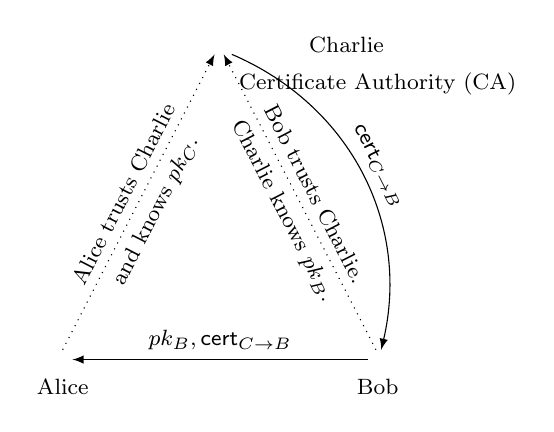
\begin{tikzpicture}[font=\footnotesize]
\node (A) at (0,0) [label=below:Alice] {\Alice};
\node (B) [right of = A, node distance = 4cm,label=below:Bob] {\Bob};
\node (KDC) at (2,4) [rounded corners=1ex,minimum width=2cm,label distance=-2cm,label=right:Charlie] {\Bob};
\node at (4,3.5) {Certificate Authority (CA)};  
\draw[-latex] (B) -- (A) node [midway,above] {$pk_B, \mathsf{cert}_{C\to B}$};
\draw[-latex,dotted] (A.90) -- (KDC.240) node [sloped,midway,above] {Alice trusts Charlie} node [sloped,midway,below] {and knows $pk_C$.};
\draw[-latex] (KDC.320) to [bend left=40] node [sloped,midway,above] {$\mathsf{cert}_{C\to B}$} (B.70);
\draw[-latex,dotted] (B.100) -- (KDC.290) node [sloped,midway,below] {Charlie knows $pk_B$.} node [sloped,midway,above] {Bob trusts Charlie.};
\end{tikzpicture}